
%% This is an example first chapter.  You should put chapter/appendix that you
%% write into a separate file, and add a line \include{yourfilename} to
%% main.tex, where `yourfilename.tex' is the name of the chapter/appendix file.
%% You can process specific files by typing their names in at the 
%% \files=
%% prompt when you run the file main.tex through LaTeX.
\section{Stability}

\subsection{Laminar to Turblent Transition}

Because of the low Reynold number of paper airplane aerodynamics, we have to worry about
the persistance of the laminar boundary layer.
There is a big difference between turbulent flow and laminar boundary
layers. Laminar boundary layer doesn't respond well to an increasing
pressure gradient in the direction of flow, whereas turbulent flow does.
However, turbulent flow results in large frictional effects and can result in stalling.
This effect is illustrated in figure~\ref{fig:boundary_layer_transition}.

\begin{figure}[hl]
  \centering
    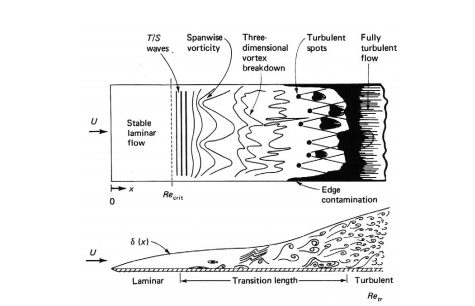
\includegraphics[scale=.5]{figures/boundary_layer_transition.png}
    \caption{This is the illustration of the transition from laminar to turbulent flow on the
    surface of an airplane. This transition is important in the design of a plane flying in
    Low Reynolds Number flow.}
  \label{fig:boundary_layer_transition}
\end{figure}

One aspect of the laminar boundary layer is the location in which it separates from the surface.
This transition region has many stages. At the first stage, unstable two-dimensional Tollmien Schlichting
waves are developed and start to move downstream. As it moves downstream, the waves become three directional
and vortical structures are formed. Finally this leads to turbulent flow.
Because of the instability this transition between turbulence and laminar flow 
can cause, predicting this location is important in the stability and other properties of the flight. 
This transition location also results in hysterisis effects. Before separation
occurs, increasing angle of attack will increase lift. But afterwards,
decreasing the angle of attack does not return to the same lift. 

One effect of laminar vs turbulence is the skin friction. When the flow is turbulent there
is a lot more skin friction then when it is laminar. The other side of it is, 
in terms of lift, maximum
lift depends on the characteristics of the turbulent boundary layer, because the
turbulent layer has the ability to recover pressure at the
rear of the airfoil.

Here are some Reynold number regimes for different boundary layers ~\cite{mueller}.

\begin{enumerate}
\item For Reynold numbers between 1000 and 10000 the boundary layer flow is laminar
and doesn't transition into trubulent flow. This type of flight is seen with
the dragon fly and the house fly. 
\item  For Reynold numbers between 10000 and 30000 the boundary layer is laminar but
it can separate. When it separates it does not reattach.
\item At 30000 to 70000 there are hysterisis effects because of the transition. 

\end{enumerate}

\subsection{Lateral Stability}

\subsubsection{Dihedral vs Anhedral}
\label{sec:dihedral}

Dihedral and anhedral refer to the angle between the wings and the horizontal plane.
Dihedral wings means that the wings point upwards, and the anhedral wings means the wings point
downwards as shown in Figure~\ref{fig:dihedraleffect}. Dihedral wings have more lateral 
stability than anhedral wings.

\begin{figure}[hl]
  \centering
    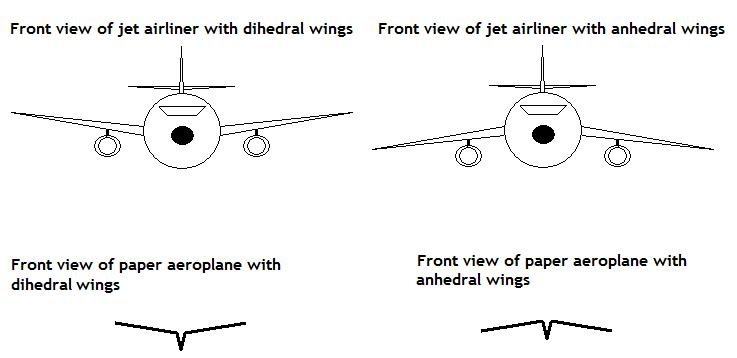
\includegraphics[scale=.5]{figures/dihedraleffect.png}
    \caption{Dihedral vs Anhedral wings}
  \label{fig:dihedraleffect}
\end{figure}

The bank angle is defined as the angle about the axis along
the plane's motion. Let us call the bank angle $\phi$. When the aircraft is
banked, this results in a rolling moment, called the dihedral effect. If the
rolling moment opposes the bank, the dihedral effect is positive. In order for
there to be stability, the dihedral effect needs to be positive. There are many
different factors that can contribute to the dihedral effect: the shape of the wings,
the wing placement, tail height, etc. We will analyze the angle of the wings in this paper.

To analyze this effect in more detail we will show that a dihedral aircraft has 
a positive dihedral effect. When the aircraft is banked we see that there is a net force
to the side, this is called sideslip (Figure~\ref{fig:dihedral1}). 
However we see that the forces on the wings do not 
contribute to the dihedral effect yet.


\begin{figure}[hl]
  \centering
    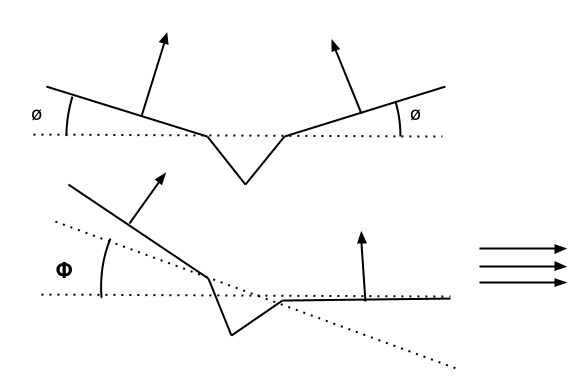
\includegraphics[scale=.5]{figures/dihedral1.png}
    \caption{SideSlip}
  \label{fig:dihedral1}
\end{figure}

At this point, with respect to the plane's frame of reference, there is air flowing 
to the side that will contribute to a dihedral effect. 
If the bank angle is $\phi$ and
the angle that the wings make with the horizontal is $\theta$ then after factoring in
the banked angle, the right wing has an angle of attack of  $\theta - \phi$.
The left wing has an angle of attack $- \theta - \phi$.
From our discussions of models of wings of airplane, we can say that the
coefficient of lift is approximately $\beta \sin(\alpha 0 \alpha_o)$.
$\alpha$ is the angle of attack and $\beta$ is a constant. To test the stability of the plane
let us assume that $|\phi| < |\theta|$.
So if we assume that $theta$ is positive , so that the airplane is dihedral.
So the left wing will experience a downward force because of a negative angle of attack
and the right wing will experience an upwards force because of a positive angle of attack, straightning the plane out.
However, if $theta$ is negative, and the plane is anhedral, the right wing will experience a
downwards force, and the left wing will experience an upwards force, increasing its lateral moment
(Figure~\ref{fig:dihedral2}). 


\begin{figure}[hl]
  \centering
    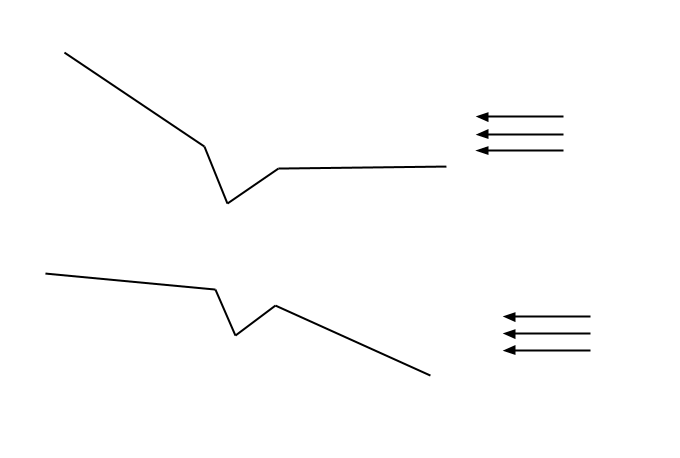
\includegraphics[scale=.5]{figures/dihedral2.png}
    \caption{Positive vs Negative dihedral effect}
  \label{fig:dihedral2}
\end{figure}


\subsection{Longitudinal Stability}
\label{sec:long_stability}

\subsubsection{Aerodynamic Center}

The Aerodynamic Center is the location on the plane where the pitching moment doesn't
change with the angle of attack. 

In order to calculate it first we will show how to 
find moments at different locations given one moment. 
Let us say we know the moment of the plane, $M_{ref}$ at some
location $x_{ref}$. Also, as an approximation, we can also say that the upwards force
is the lift and the horizontal force is the drag. We would like to find the moment
at some $x_{new}$, $M_{new}$. Let us assume that the z dimension does not contribute to the
calculations because the airplane is pretty  is thin.

\[M_{ref} = -(x_{new} - x_{ref})L + M{new} \] 

because $-(x_{new} - x_{ref})L$ is the torque. We can convert this equation into their
respective coefficients, the pitching moment coefficient, and the lift coeffiient.

\[C_{m_{ref}} = - ( \frac{x_{new} - x_{ref}}{c})C_L + C_{m_{new}} \]

Where $c$ is the average chord length.

Next let us let $M_{new}$ be the moment about the aerodynamic center and
differentiate with respect to $\alpha$.

\[\od{C_{M_{ref}}}{\alpha} = - (\frac{x_{ac} - x_{ref}}{c}\od{C_L}{\alpha}) + (\od{C_{M_{ac}}}{\alpha})\].

By definition 
\[\od{C_{M_{ac}}}{\alpha} = 0\]

Therefore we can solve for $x_ac$ and we obtain:

\[\frac{x_{ac} - x_{ref}}{c} = \frac{x_{ref}}{c} - (\od{C_{M_{ref}}}{C_L})\]

Therefore, if we know the moment at one point, and we can figure out the derivative 
$\od{C_{M_{ref}}}{C_L}$. It has been found theoretically that this moment
occurs at a quarter of a chord back from the leading edge on most airfoils ~\cite{NASAac}.



\subsection{Wing Stability}
Let $\alpha$ be the angle with the horizontal. Also,
$C_M$ be the moment at the center of gravity.  In order for a plane to have static
stability:

\begin{equation}
C_M = 0
\end{equation}
\begin{equation}
\od{C_M}{\alpha} < 0
\label{eq:long_stability}
\end{equation}

As we have shown in our models, the lift coeffient is a linear function of $\alpha$, therefore
we can conclude that the condition is:

\[\od{C_M}{C_L} < 0 \]

To figure out the moment of the plane we start by figuring out the moment of the wings.
There are only two forces on the wings, the lift force and the drag force. Let us say
that the angle between the air flow and the airplane is $\alpha_{FRL}$ to the plane as shown in the picture below 
FIgure~\ref{fig:longitudinal_stability1}.

\begin{figure}[hl]
  \centering
    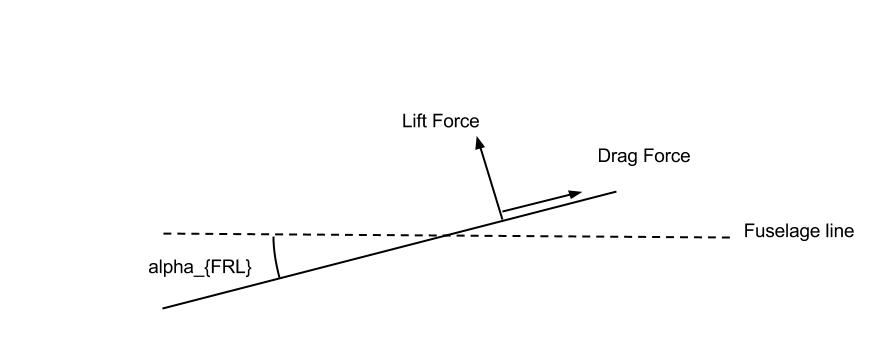
\includegraphics[scale=.5]{figures/longitudinal_stability1.png}
    \caption{Longitudinal Wing Stability}
  \label{fig:longitudinal_stability1}
\end{figure}

From the formula from the previous section, we see that 

\[M_{cg}  = -(L\cos(\alpha_{FRL}) + D\sin(\alpha_{FRL}))(x_{cg} - x_{ac}) + M_{ac}\]

Again we will assume that the z component does not contribute. Then we change it into
coefficient form once more and use a small angle approximation.

\[ C_{M_{cg}} = -(C_{L} + C_D \alpha_{FRL}) (\frac{x_{cg}}{c} - \frac{x_{ac}}{c}) + C_{M_{ac}} \]

Because $\alpha_{FRL}$ is small we can approximate $C_{M_{cg}}$ as

\[-C_L (\frac{x_{cg}}{c} - \frac{x_{ac}}{c}) + C_{M_{ac}} \]

Because the aerodynamic center has no dependence on $\alpha_{FRL}$ we can rewrite the
stabiltiy equation as:

\[\od{C_{M_{cg}}}{C_L} = - \frac{x_{cg}}{c} + \frac{x_{ac}}{c} < 0\]

Therefore, the bigger $x_{cg}$ is the more stable the plane is. By our choice of coordinate system,
this means that the center of mass of the plane has to be in front of the aerodynamic center for it to have
longitudinal stability.

              

